\documentclass[french]{article}
\usepackage{graphicx}
\usepackage{caption}
\usepackage[T1]{fontenc}
\usepackage[utf8]{inputenc}
\usepackage{lmodern}
\usepackage{geometry}
\geometry{
	a4paper,
	left=25mm,
	right=25mm,
	top=30mm,
	bottom=30mm,
}
\usepackage{babel}
\usepackage{pgfgantt}
\usepackage{eurosym}

\usepackage[babel=true, kerning=true]{microtype}

\usepackage{subcaption}

\usepackage[unicode=true,pdfusetitle,bookmarks=true,bookmarksnumbered=false,bookmarksopen=false,
breaklinks=false,pdfborder={0 0 0},backref=false,colorlinks=true,urlcolor=blue]{hyperref}

\graphicspath{{images/}}

\author{Andrea Brugnoli \\ 
\hspace{2.8pt} Docteur ISAE-Supaéro 2020\\
Ingénieur ISAE-Supaéro 2017}
\title{Méthodes numériques respectueux de la physique: de la modélisation multi-physique haute fidélité aux modèles réduits pour l'ingénierie}

\date{}

\begin{document}

\maketitle

\large{Dossier de candidature au prix de la fondation Jean-Jacques et Félicia
	Lopez-Loreta pour l’excellence académique}


\begin{figure}[h]
	\centering
	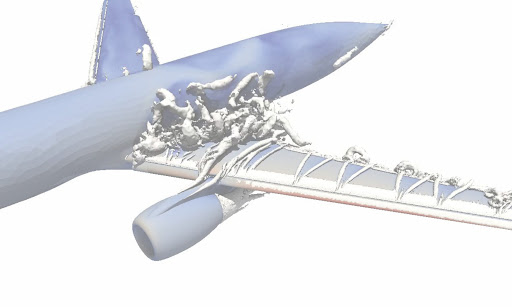
\includegraphics[width=.95\textwidth]{3Dplane.jpg}
	\captionsetup{labelformat=empty}
	\caption{Source: \href{http://www.fenics-hpc.org/}{FEniCS-HPC website}}
\end{figure}





\thispagestyle{empty}

\newpage

\section{Contexte et objectifs du projet}

\subsection{Le candidat}


La technologie,  les sciences et leur impact sur l'humain m'ont toujours intéressé. C'est pour cela que j'ai opté pour un baccalauréat littéraire avec option informatique (obtenu en 2011 \`a Vérone, Italie). Après mon baccalauréat\footnote{En Italie il est possible d'accéder aux universités scientifique après un Bac. L.}, j'ai obtenu une licence en ingénierie mécanique du Politecnico de Milan. Pendant la première année du master en ingénierie Spatiale, j'ai décide de partir \`a l'étranger et j'ai choisi d'effectuer un double diplôme \`a l'ISAE-SUPAERO. J'ai pu approfondir mes connaissances en automatique grâce \`a un Master Recherche en collaboration avec Supélec/Université Paris Saclay, ainsi que mes compétences en mathématiques appliquées \`a travers un parcours spécialisé. Mon intérêt pour les systèmes dynamiques et la simulation m'a amené au centre national d'études spatiales (CNES) pour mon stage de fin études, o\`u j'ai effectué des simulations intensives sur le supercalculateur. \\

J'ai donc décidé de poursuivre un doctorat de recherche en automatique et mathématiques appliquées (calcul numérique), au sein du projet ANR-DFG INFIDHEM (Interconnected Infinite-Dimensional Systems for Heterogeneous Media). Le projet consistait \`a utiliser un formalisme mathématique capable de traiter d'une manière unifiée les problèmes multi-physiques. Mon travail était centré sur la modélisation et discrétisation des structures flexibles minces, très utilisées dans l'aéronautique (cf. Fig \ref{fig:IntRod}). Mes travaux de thèse ont été présentés devant un jury international (Thomas Hélie, directeur de Recherches DR2 au CNRS, Yann Le~Gorrec, Professeur ENSMM et Alessandro Macchelli, professeur associé \`a l'Universit\'e de Bologne) et ont été diffusés au travers de conférences internationales et de 5 articles de revue rédigés par le candidat \cite{brugnoli2019ammmin,brugnoli2019ammkir,brugnoli2020msd,brugnoli2021ther,brugnoli2021num}. \\

Ma forte curiosit\'e pour les thématiques de ma thèse ne m'a pas abandonné par la suite. C'est pour cela que j'ai décidé de continuer en Post-Doc \`a l'Universit\'e de Twente aux Pays Bas, au sein d'un projet qui vise \`a étendre la compréhension des mécanismes physiques sous-jacents au vol biologique (en particulier les oiseaux). Mon rôle consiste \`a mettre en place des algorithmes numériques capables de reproduire fidèlement la structure physique du problème \cite{califano2021}.

\begin{figure}[h]
	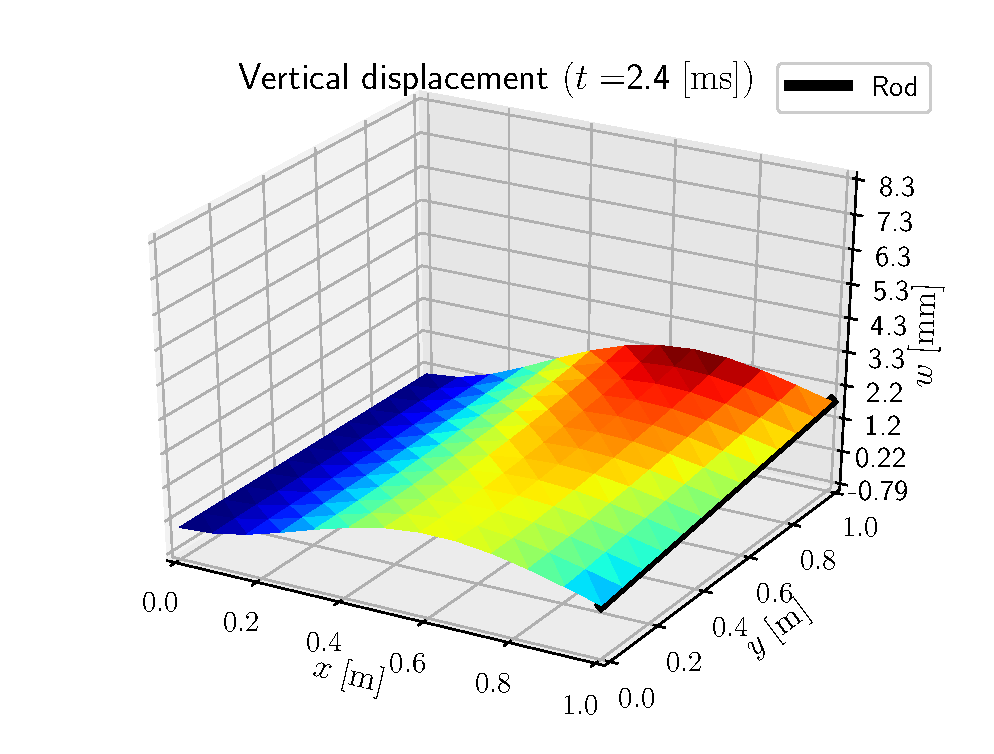
\includegraphics[width=0.45\linewidth]{SnapRod_t25.eps}
	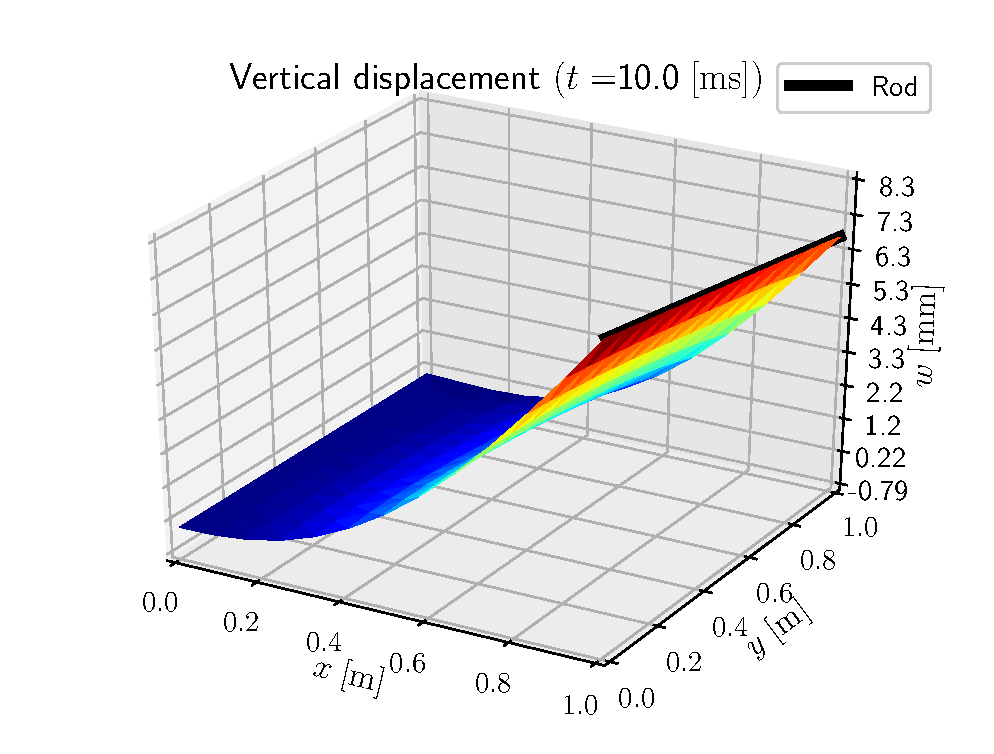
\includegraphics[width=0.45\linewidth]{SnapRod_t100.eps}
	\caption{Simulation d'une plaque mince flexible connectée \`a une poutre rigide.}
	\label{fig:IntRod}
\end{figure}


\subsection{Contexte}


Ma thèse s'est inscrite dans le cadre d'un projet européen financé par l'agence national de la recherche (ANR) et la Fondation allemande pour la recherche (DFG). L'ambition du projet était de pousser la compréhension d'un formalisme mathématique issu de la physique et de la théorie des systèmes pour le traitement unifié de divers domaines d'applications (mécanique des solides, des fluides, l'électromagnétisme et la thermodynamique). Il s'agit du formalisme port-Hamiltonien, bas\'e sur la mécanique Hamiltonienne et les graphes de liaisons pour la modélisation des systèmes dynamiques. Il y a 30 ans, le premier article sur cette théorie était publié. Dans le cadre de ma thèse, j'ai pu contribuer \`a étendre ce formalisme vers les applications, en développant des modèles mathématiques et numériques pour la mécanique des structures flexibles \cite{brugnoli2019ammmin,brugnoli2019ammkir}, la mécanique multi-corps flexibles~\cite{brugnoli2020msd} et la thermoelasticit\'e~\cite{brugnoli2021ther}. \\

Aujourd'hui ce formalisme a désormais atteint le niveau de maturit\'e nécessaire pour attaquer les applications industrielles. Le professeur Volker Mehrmann, vice-président de la société mathématique européenne (EMS), en est pleinement convaincu, et il a récemment illustré les avantages de cette approche  lors de la SIAM Conference on Computational Science and Engineering en 2021\footnote{\url{https://meetings.siam.org/sess/dsp_programsess.cfm?SESSIONCODE=70329}}. Ce niveau de maturit\'e est aussi attesté par le fait que le conseil de la recherche européen (ERC) \`a récemment attribu\'e au Prof. Stefano Stramigioli une subvention de 2.8 millions \euro{} pour le projet Portwings\footnote{\url{http://www.portwings.eu/}}. Ce projet, dans le quel je suis impliqu\'e pour mon post-doctorat, cherche \`a améliorer la compréhension du vol battu pour pouvoir perfectionner le design et la construction des robots biomimétiques. L'ambition réside dans le fait d'utiliser la théorie port-Hamiltonienne pour expliquer les interactions complexes entre l'aérodynamique et la flexibilit\'e de l'aile (cf. Fig. \ref{fig:pH_view_bird}). \\

Pour réaliser un développement substantiel dans les domaines d'application les plus critiques pour la société, des investissements considérables seront nécessaires dans les méthodes mathématiques et informatiques : il faudra disposer  de techniques de déploiement robustes, rapides et accessibles \cite{niederer2021}. Étant donné le potentiel du formalisme port-Hamiltonien pour les traitement unifié des problèmes multiphysiques \`a travers différentes échelles et précision, il est possible que son adoption en industrie soit de nature \`a faciliter cette révolution digitale. 

\begin{figure}[tb]
	\centering
	\includegraphics[width = .7\textwidth]{Bird_Port_Hamiltonian_Subsystems_FULL_ARC.eps}
	\caption{Modèle d'un oiseau robotique bio-inspiré.}
	\label{fig:pH_view_bird}
\end{figure}

\subsection{Le projet}
Dans ce projet de recherche, le but consiste \`a mettre en place des méthodes numérique pour accélérer la simulation des problèmes fluide-structure d'un facteur 100, par rapport au temps de calcul demandé par une simulation haute-fidélité.  La réussite du projet permettra donc d'intégrer des modèles physique plus économiques, qui pourront remplacer des simulations très co\^{u}teuses, et ainsi de faciliter le design et la prise des décisions. Différemment des plusieurs méthodes proposes dans la littérature, dans ce projet l'impératif reste la fidélité \`a la physique \cite{willcox2021}. Le formalisme port-Hamiltonien représente un candidat idéal a fin de atteindre ce but. \\

La vision qui sous-tend ce projet est que l'utilisation d'algorithmes fidèles \`a la structure physique du problème pourra radicalement améliorer les techniques normalement utilisées pour la réduction des modèles et l'optimisation. La structure physique du problème est le plus souvent ignorée par les algorithmes de réduction, qui traitent les simulations comme des bo\^{i}tes noires. Le modèles réduits respectueux de la physique sont extrêmement plus précis des ceux qui ne garantissent pas le respect de la physique sous-jacente \cite{lee2020}. 


\section{Aspects innovants du projet et verrous scientifiques}

\subsection{État de l'art}
La cout prohibitif des simulations numériques des problèmes couplée fluides-structure a poussé la communauté scientifique a concevoir des algorithme capable de réduire la complexité des modèles. La vaste majorité des ces méthodes assument que on puisse obtenir un système réduit \'a travers une méthode essentiellement linéaire, i.e. la Décomposition Orthogonale aux Valeurs Propres \cite{shinde2019,tello2020fluid}. Cette hypothèse n'est pas valable pour tout systèmes exhibant un comportement non linéaire et amène à surestimer la dimensionnalité du système réduit \cite{kerschen2005}. Grâce aux progrès récents dans le domaine de l'intelligence artificielle, des nouvelle méthodes permets d'obtenir des modèles réduits rapides. Certains méthodes utilisent les données issues des simulations fines \cite{lee2020}, d'autres ne demandent pas des simulations couteuses, mais cherchent \'a minimiser la violation des principes physiques~\cite{sun2020physics}.  
Tout ces méthodes ne garantisses pas le respect de la structure physique dans toute la chaine qui amène au modèle finale. Ce projet va essayer de respecter la structure physique dans toutes les étapes, comme expliqué dans le paragraphe qui suit.


\subsection{Verrous scientifiques}


Le premier défi du projet consiste a implémenter des méthodes numérique pour la résolution des systèmes couplés multiphysique. Ces modèles numériques devront retenir les propriétés physiques du problème (conservation d'énergie globale, traçage des échanges d'énergies entre différents systèmes, conservation d'invariants du problème). En industrie normalement différent méthodes sont utilisées pour simuler différentes physiques. Par conséquence, le couplage numérique ne représente pas correctement les fluxes d'énergie. L'utilisation d'un paradigme de modélisation unifié permettra donc d'effectuer les couplage d'une manière à respecter la physique. \\

Le second challenge du projet consiste à intégrer des technique issues de l'Intelligence Artificielle seront utilisées pour obtenir des modèles réduit. Dans cette phase, il sera important de préserver la structure du problème en sors d'obtenir un modèle réduit fidèle à la physique. Une technique très prometteuse en ce sens est présentée dans \cite{lee2020}, mais ici le respect des lois physiques est imposé à posteriori à travers de contraintes et non pas inclus au niveau de la structure.

Le dernier objectif consistera \`a utiliser ces modèles réduits pour optimiser le design mécanique des structures et vérifier la validité des modèles réduit.  Cette étape permettra d'évaluer la validité et l'efficacit\'e des modèles réduits par rapport aux simulations fines. \\


Les modèles réduit seront plus rapides mais inévitablement moins précis par rapport aux simulations fines. Venir à bout de ces trois macro-tâches permettra de comprendre le compromis entre temps de calcul et précision pour des applications d'intérêt industriel. 

\subsection{Domaines d'application}

Au delà de l'aéronautique, ou l'aéroélasticité reste un challenge essentiel, différents secteurs d'applications pourront bénéficier des outils développes dans le cadre de ce projet (cf. Fig {fig:applications}): \\
\begin{itemize}
	\item En robotique les chercheurs cherchent de plus en plus d'imiter la nature. Cela a permit de réaliser des drones reproduisant des oiseux, des insectes et des poissons. Pour pouvoir améliorer les performances des ces drones à travers grâce au contrôle en temps réel, il est nécessaire de disposer des modèles faciles à simuler. 
	\item Pour réduire les couts associée a la maintenance des réseaux de distribution (énergie électrique, gas, hydrogène ou hydraulique), des méthodes structurés capable de représenter une hiérarchie des modèles sont nécessaire. Le cout computationelle est trop élevé pour pouvoir optimiser ces modèles directement.
	\item Afin de fournir des services Internet dans des endroits sans accès haut débit, une solution prometteuse consiste à utiliser des constellation des satellites équipés des antennes constitue des différents modules réflecteurs (reflectarray). Pour concevoir ces modules, des modeles intégrants l'électromagnétisme et la thermomécanique sont nécessaires.
\end{itemize}






\begin{figure}
	\begin{subfigure}[t]{0.25\textwidth}
		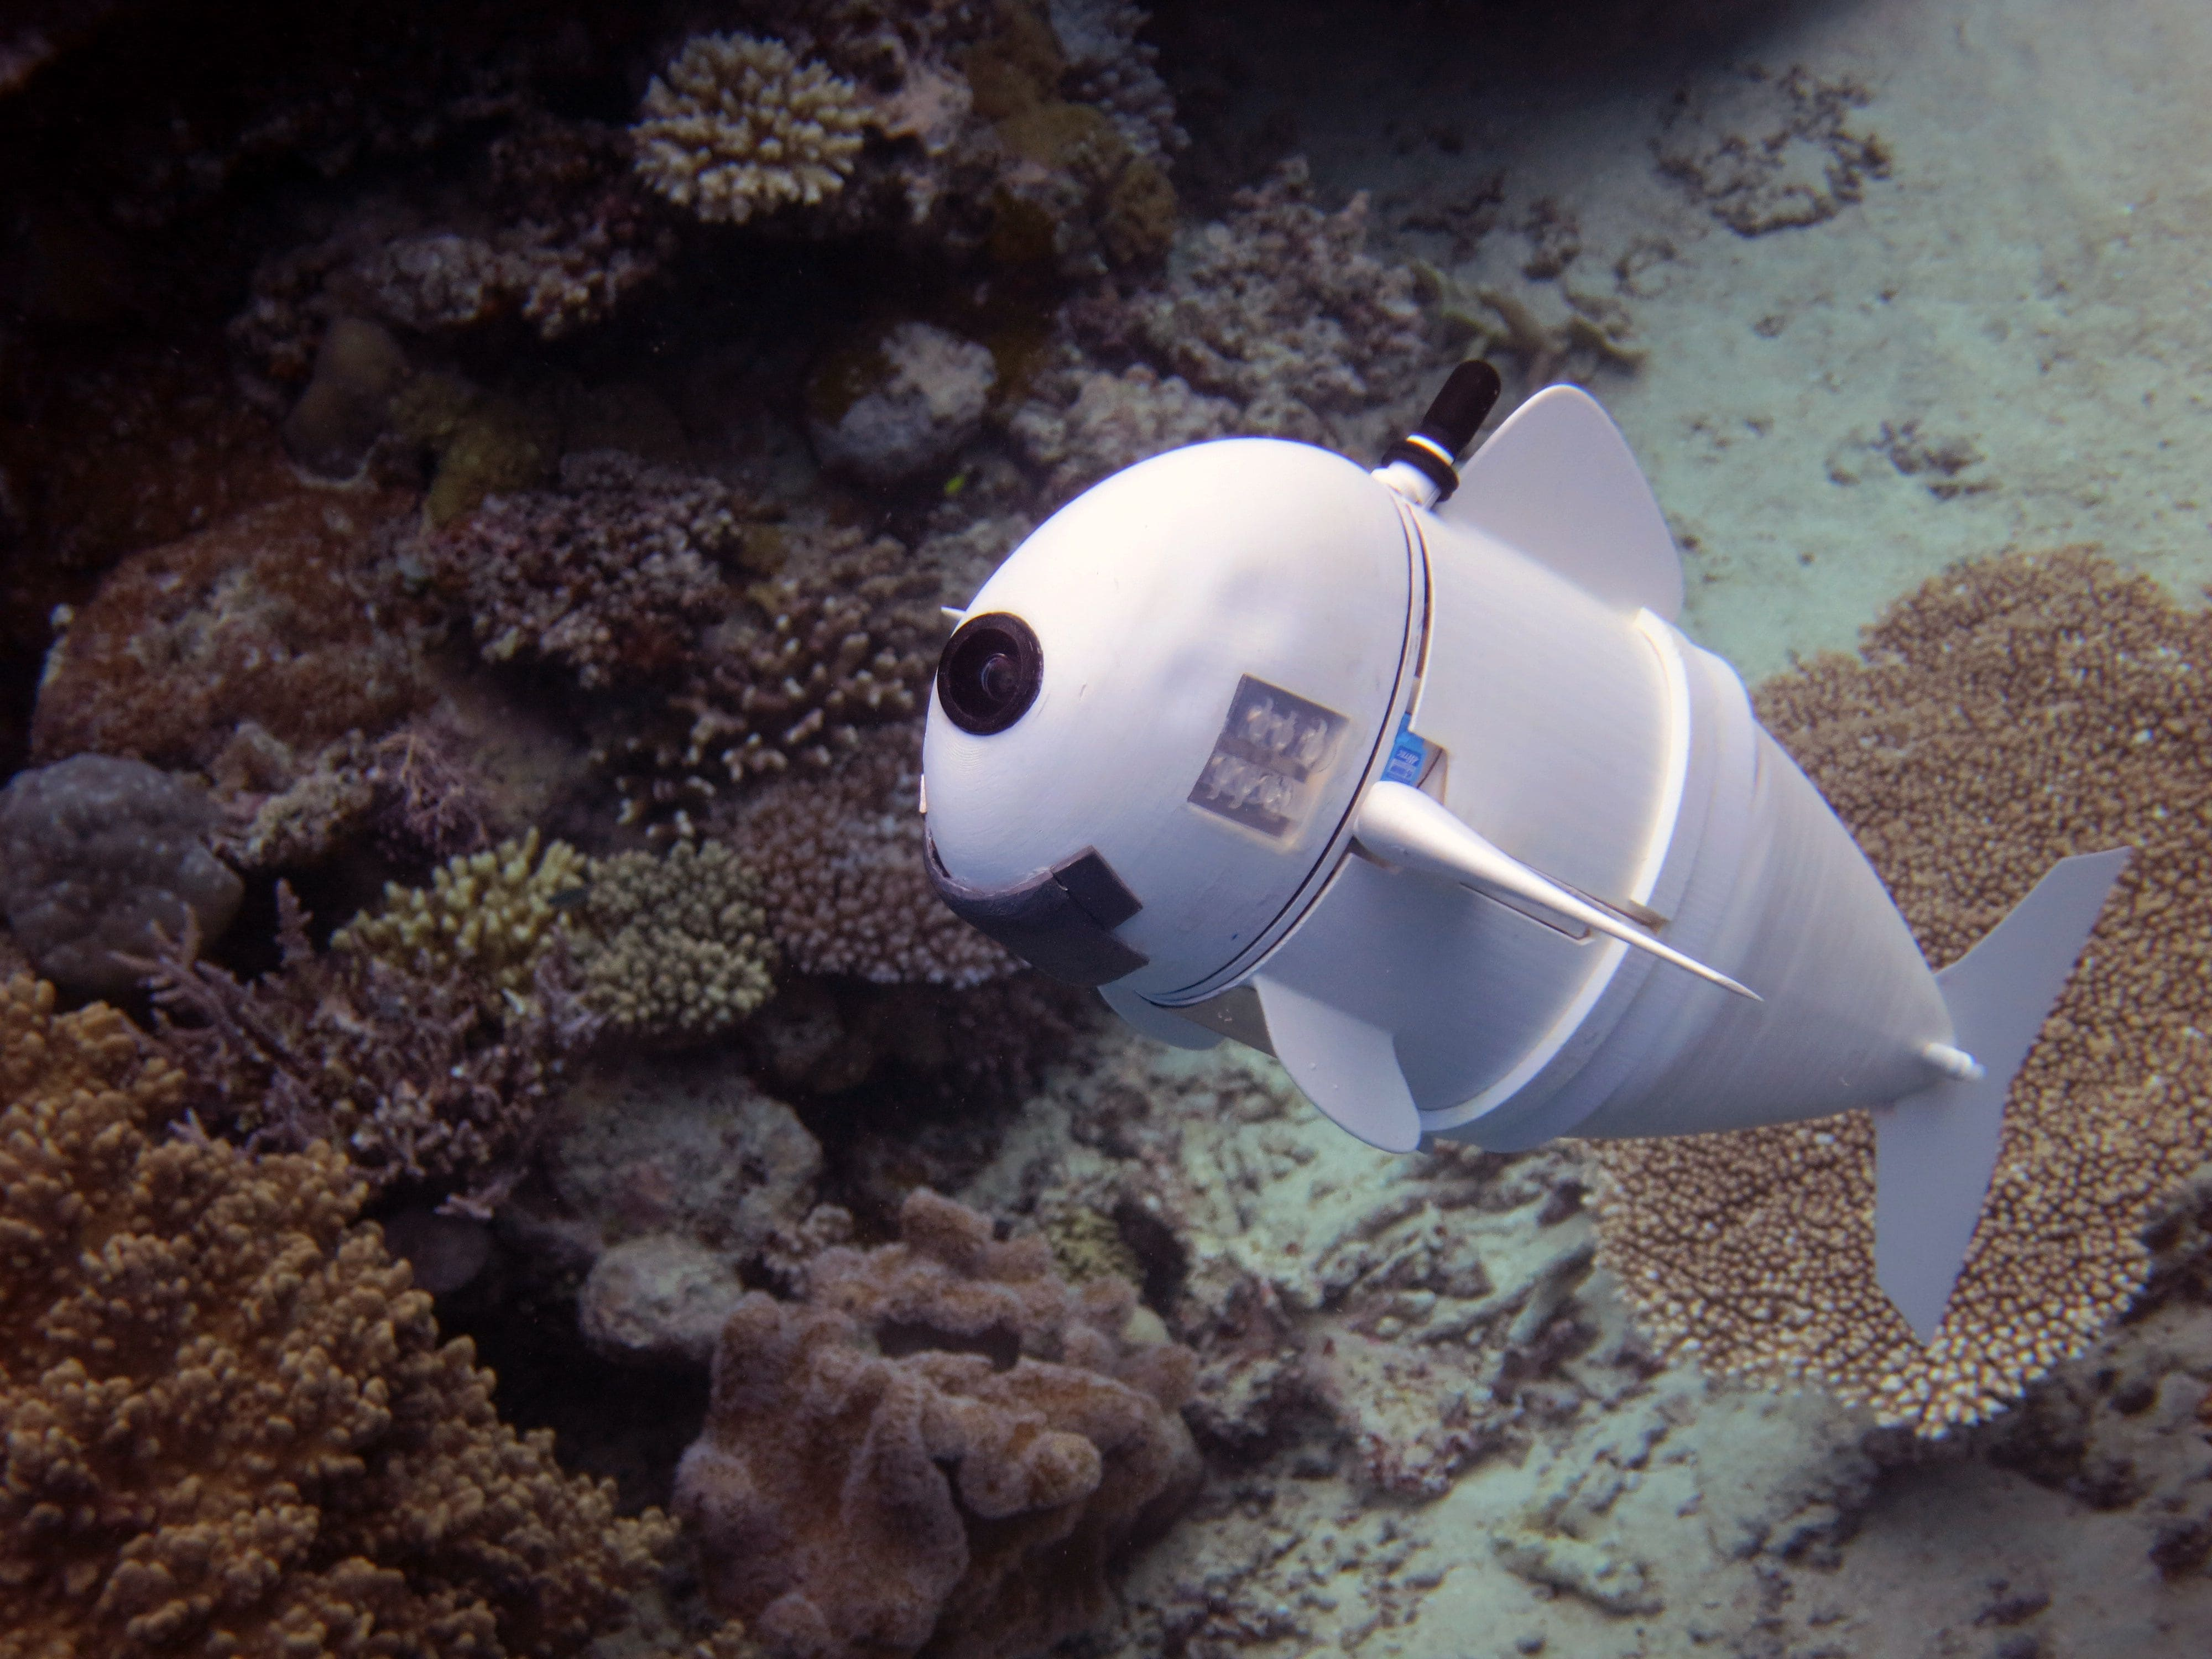
\includegraphics[width=\columnwidth]{Sofi_MIT.jpeg}%
		\caption{Le robot SoFi (MIT)}
		\label{fig:sofi-mit}
	\end{subfigure}\hfill
	\begin{subfigure}[t]{0.25\textwidth}
		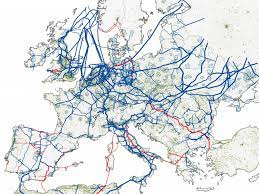
\includegraphics[width=\columnwidth]{EU_gas_network.jpeg}%
		\caption{Réseau européen du gaz}
		\label{fig:network}
	\end{subfigure}\hfill
	\begin{subfigure}[t]{0.35\textwidth}
		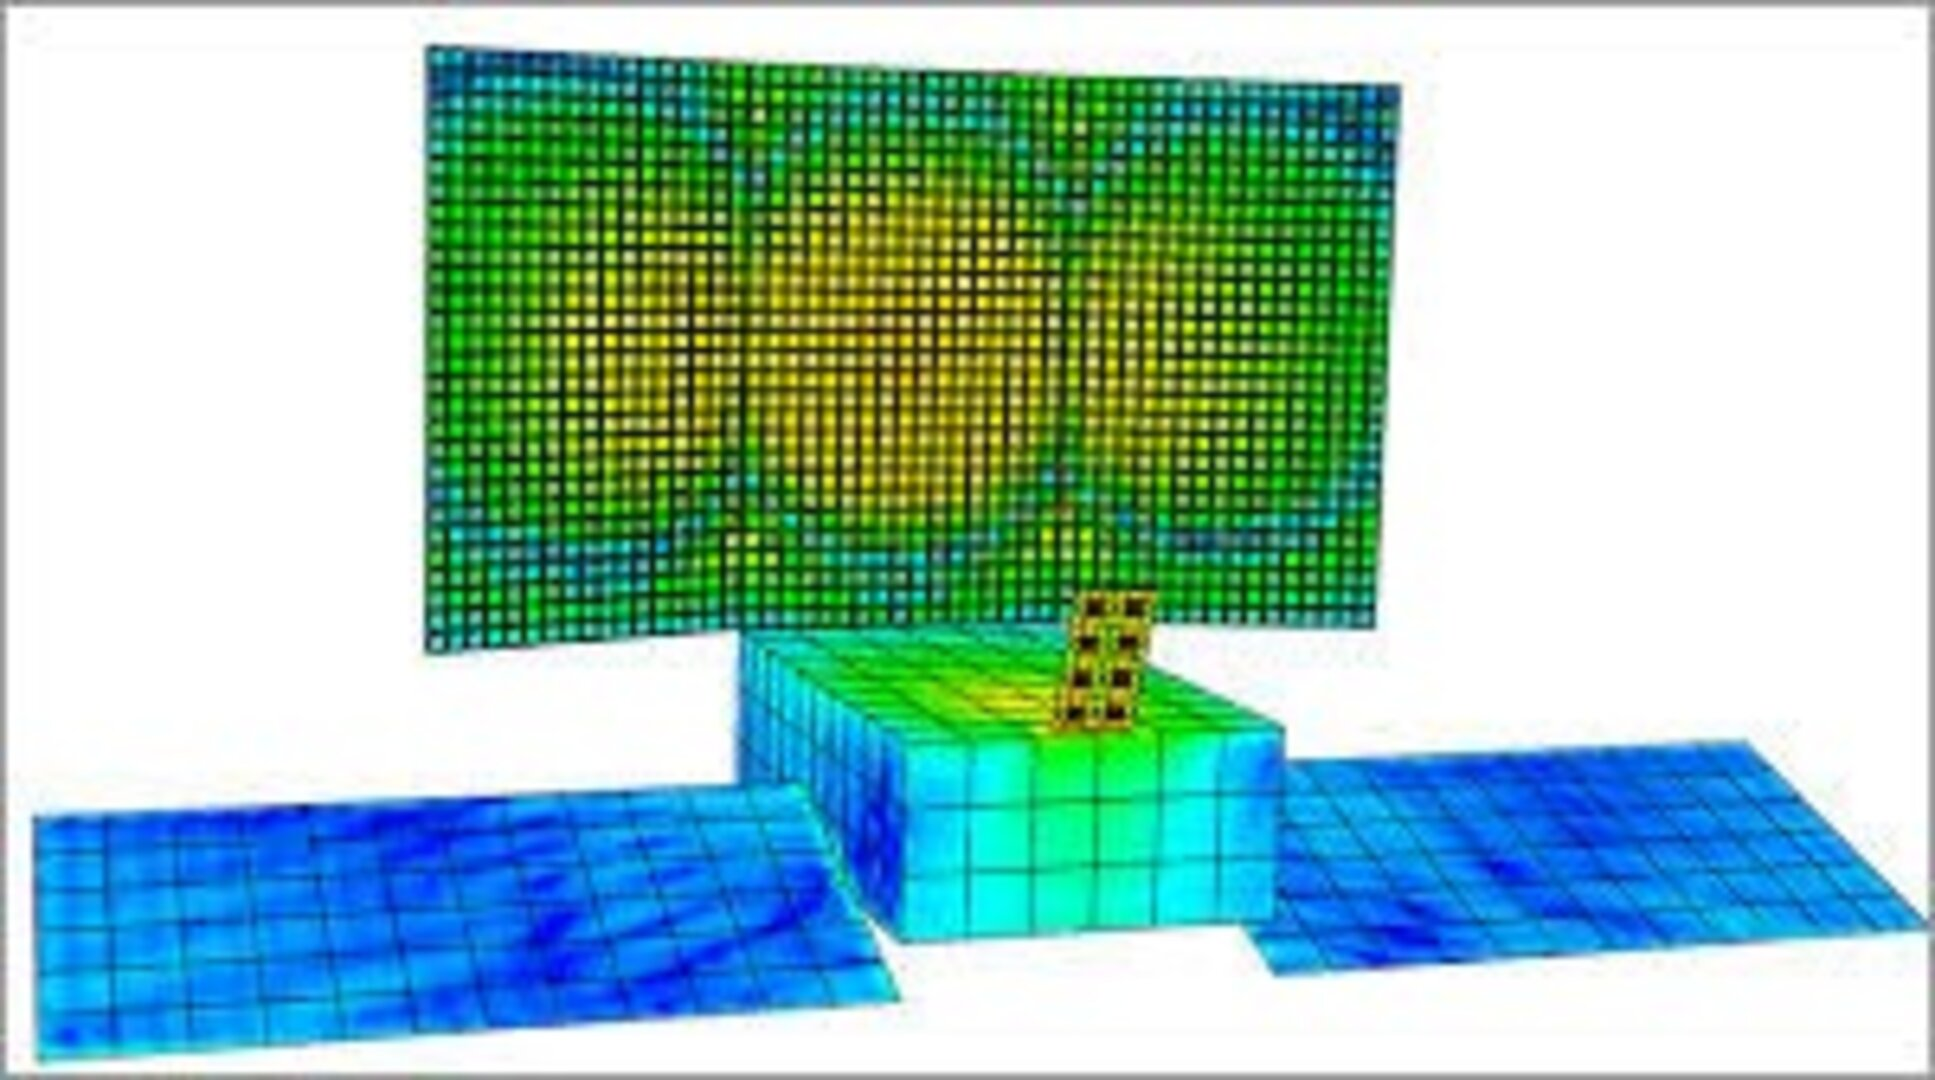
\includegraphics[width=\columnwidth]{Reflectarray.jpg} 
		\caption{Logiciel simulation antenne reflectarray (ESA)}
		\label{fig:array}
	\end{subfigure}%
	\caption[]{Exemple des cas d'application des outils computationelle développés dans le cadre de FLUSI \footnotemark}%
	\label{fig:applications}%
\end{figure}



\footnotetext{Sources : \\
\url{https://www.csail.mit.edu/research/sofi-soft-robotic-fish} \\
\url{https://vividmaps.com/the-european-natural-gas-network/} \\
\url{https://www.esa.int/Enabling_Support/Space_Engineering_Technology/Smart_design_of_flat_reflectarray_satellite_antennas}
}


\subsection{Portée du projet}

Les modèles ainsi obtenus pourront être utilisés pour réduire les  co\^{u}ts associés au design, \`a l'optimisation et \`a l'inspection en cours de vie.

\section{Organisation du projet}
Le projet est divisé en trois work packages :

\begin{enumerate}
	\item Développement d'algorithmes numériques haute-fidélité pour des problèmes d'interaction fluide-structures.
	\item Méthodes de réduction garantissant le respect de la structure physique. 
	\item Utilisation des modèles réduits pour l'optimisation multidisciplinaire et comparaison avec modeles haute-fidelité.
\end{enumerate}

Chaque macro-tâche est directement associ\'ee \`a une thèse. Pour cela les recrutements des trois doctorants et d'un post-doctorant sont prévus, ainsi que la coopération des trois chercheurs. Chacun d'entre eux sera affecté \`a chaque macro-sujet:
\begin{itemize}
\item développement du code pour calcul scientifique;
\item développement du code pour la partie intelligence artificielle;
\item expertise pour l'optimisation multidisciplinaire.
\end{itemize} 
\begin{figure}[h!]
	\begin{center}
	\begin{ganttchart}[y unit title=0.6cm,
		y unit chart=0.6cm, 
		x unit=0.4cm,
		vgrid,hgrid, 
		title label anchor/.style={below=-1.6ex},
		title left shift=.05,
		title right shift=-.05,
		title height=1,
		progress label text={},
		bar height=0.7,
		group right shift=0,
		group top shift=.6,
		group height=.4]{1}{30}
		%labels
		\gantttitle{Dur\'ee totale}{30} \\
		\gantttitle{$T_0 + 12$}{6} 
		\gantttitle{$T_0 + 24$}{6} 
		\gantttitle{$T_0 + 36$}{6} 
		\gantttitle{$T_0 + 48$}{6} 
		\gantttitle{$T_0 + 60$}{6} \\
		%tasks
		\ganttbar{Partenariats}{1}{2} \\
		\ganttbar{Code SCRIMP}{1}{1} \\
		\ganttbar{1$^\circ$ th\`ese}{4}{21} \\
		\ganttbar{2$^\circ$ th\`ese}{10}{27} \\
		\ganttbar{3$^\circ$ th\`ese}{13}{30} \\
		\ganttbar{Post-Doc}{16}{27} \\
		\ganttbar{Soutenances}{22}{30} \\
		\ganttbar{Dissémination}{28}{30} 
		%relations 
		\ganttlink{elem0}{elem2} 
		\ganttlink{elem1}{elem2} 
		\ganttlink{elem1}{elem3} 
		\ganttlink{elem1}{elem4} 
		\ganttlink{elem1}{elem5}
		\ganttlink{elem2}{elem5}
		\ganttlink{elem3}{elem5}
	\end{ganttchart}
	\end{center}		
\end{figure}

\`A la fin du projet, le livrable consistera en un code capable de modéliser des problèmes multiphysiques et de générer des modèles réduits utilisables en lieu et place des modèles haute fidélité.

\subsection{Moyens et partenariats}
Pour ce que il concerne la mise en place du projet, des différents partenariats en France et \`a l'international seront mis en place. Pour ce qui concerne les aspect théoriques fondamentaux Bernhard Maschke (Universit\'e de Lyon), Arjan van der Schaft (University of Groningen) et Stefano Stramigioli (University of Twente) constitueront les interlocuteurs académiques principaux. \\

Pour ce qui concerne la première macro-tâche, il sera possible de prolonger le travail effectué dans le cadre de ma thèse, qui a donn\'e lieu a un code de calcul pour application multiphysique (le code SCRIMP décrit dans~\cite{brugnoli2021num}). Ce code sera ultérieurement développé pour traiter des problèmes d'interaction fluide-structure. Pour ce qui concerne la préservation de la physique au sein des algorithmes, des collaborations avec Marc Gerritsma (département d'aérodynamique de l'Universit\'e de Delft) et Herbert Egger (Johannes Kepler University Linz) seront mises en place. Pour ce qui concerne l'interaction fluide-structure, l'office National d'Études et de Recherches Aérospatiales (ONERA), garant d'une profonde expertise en ce domaine, représentera l'interlocuteur principal pour les problèmes liés au couplage multiphysique. 
\\


Pour ce qui concerne la deuxième macro-tâche, i.e. la réduction des modèles, il sera possible de mettre en place des collaboration avec Charles Poussot-Vassal (chercheur principal \`a l'ONERA),  Volker Mehrmann (TU Berlin) et George Haller (ETH Zurich). \\

Pour la troisième partie, il sera important de dialoguer avec Joseph Morlier (ISAE-Supa\'ero et Institut Clément Ader).


\subsection{Budget}
\begin{center}
\begin{tabular}{|c|c|}
	\hline
	D\'epense & Co\^{u}t \\
	\hline
	Porteur du projet (temps plein) & $5\times 65000=3250000$ \\
	3 doctorants (temps plein) & $3\times 3\times 40000=360000$  \\
	1 Post-Doc (temps plein) & $2\times 55000=110000$ \\
	Personnels ISAE & $100000$ \\
	Matériel  et calcul HPC & $60000$ \\
	Frais annexes (conférences, workshops) & $45000$ \\
	\hline
	\textbf{Total} & 1000000 \\
	\hline
\end{tabular}
\end{center}



\footnotesize
\bibliographystyle{unsrt}
\bibliography{biblio_articles}

\end{document}
